\section{Diabetic patient analysis}
\graphicspath{{img/diabetes/}}
\frame{\frametitle{An overview}
    \centering
    \begin{minipage}{.6\linewidth}
        \makebox[\linewidth]{%
            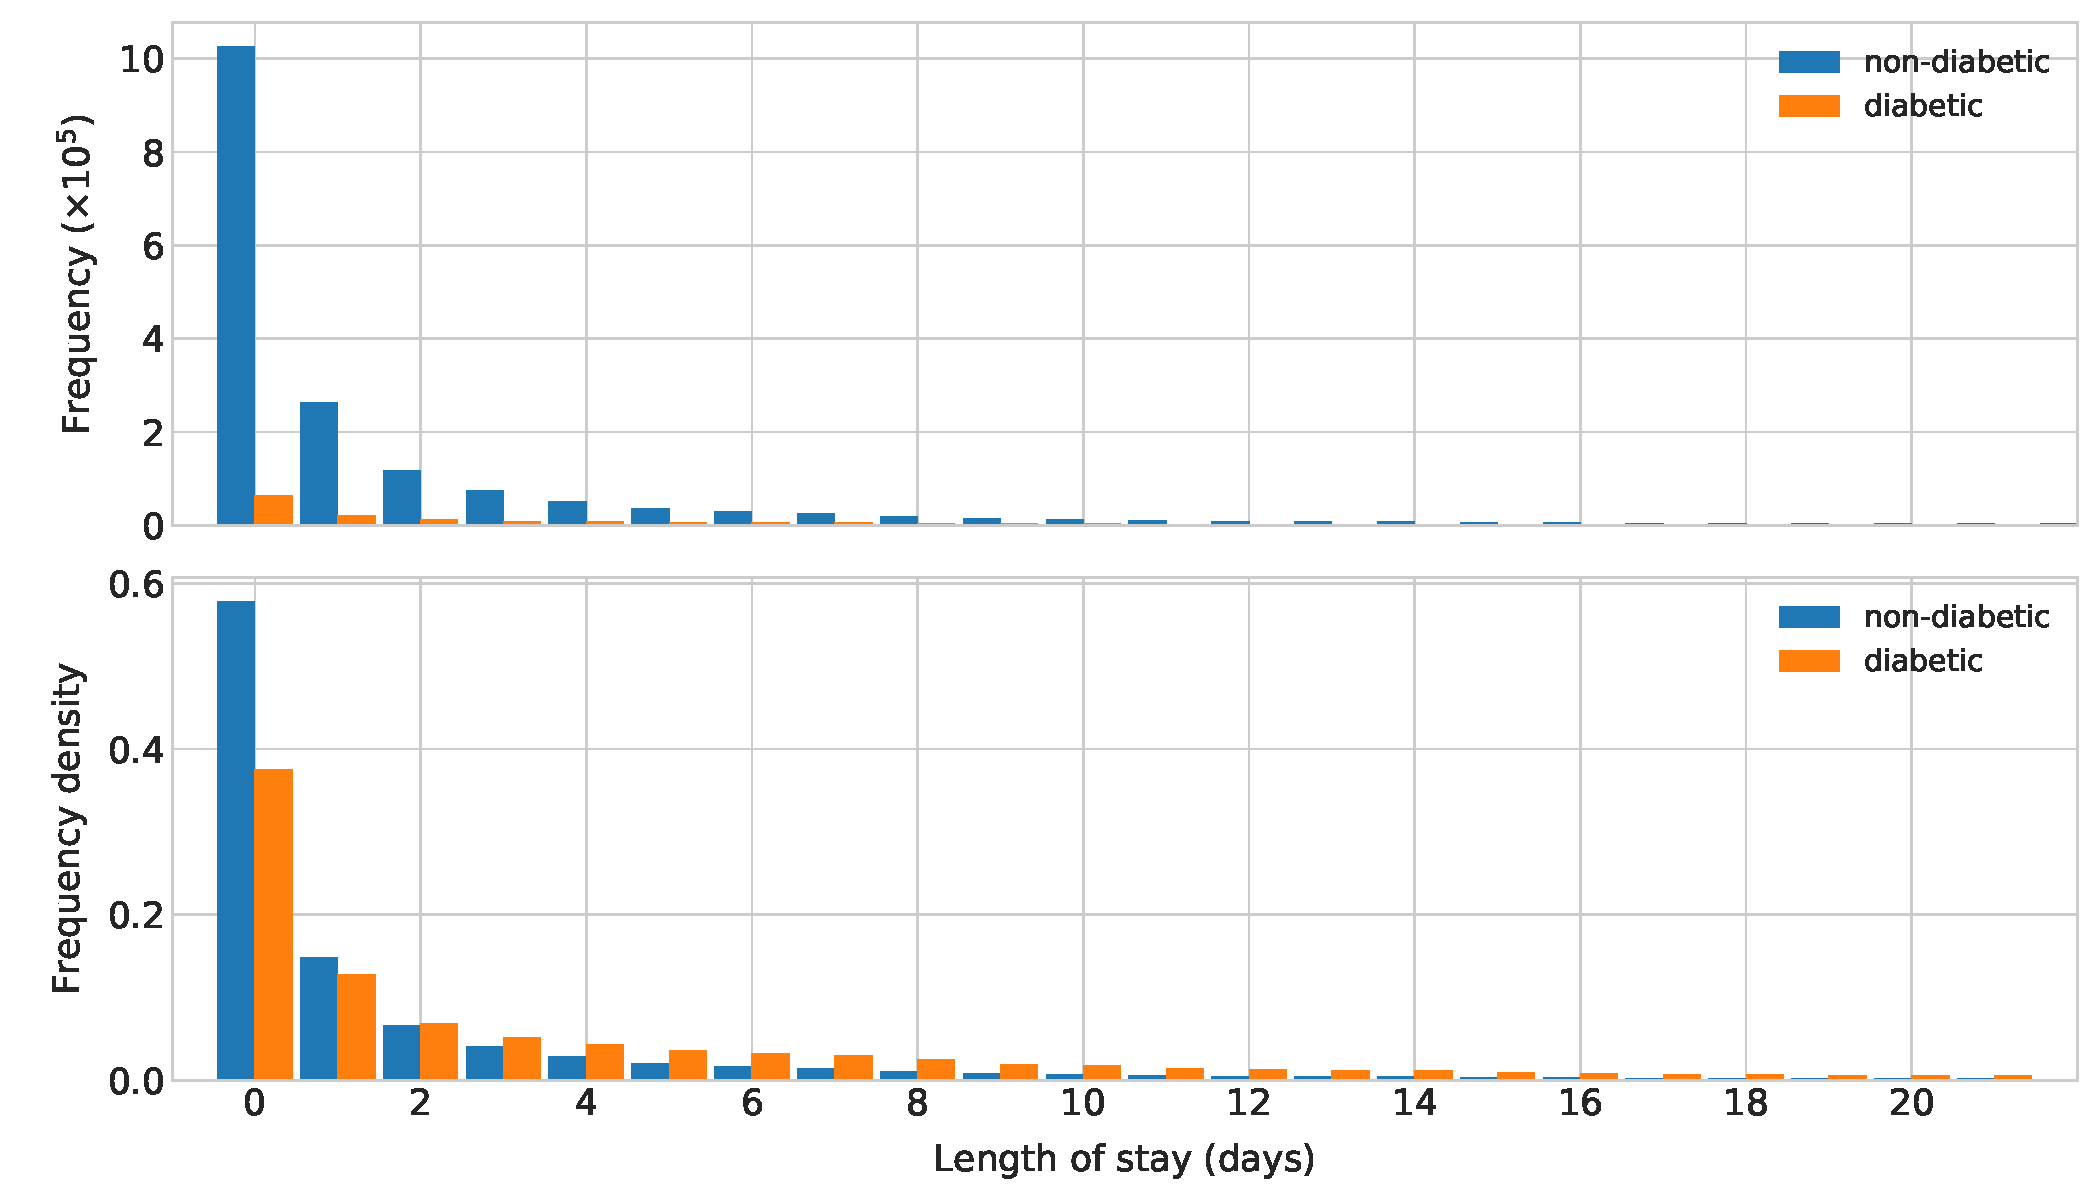
\includegraphics[width=\linewidth]{los_bar.pdf}
        }
    \end{minipage}\hfill%
    \begin{minipage}{.3\linewidth}
        \centering
        \textbf{\tiny{Length of stay}}
        \resizebox{\linewidth}{!}{%
            \begin{tabular}{lll}
\toprule
{} & Non-diabetic & Diabetic \\
\midrule
mean &         2.57 &     6.07 \\
std  &         8.13 &    12.55 \\
min  &         0.00 &     0.00 \\
1\%   &         0.00 &     0.00 \\
25\%  &         0.00 &     0.00 \\
50\%  &         0.00 &     1.00 \\
75\%  &         2.00 &     7.00 \\
99\%  &        35.00 &    57.00 \\
max  &       690.00 &   705.00 \\
\bottomrule
\end{tabular}

        }
    \end{minipage}\hfill%

    \begin{minipage}{.6\linewidth}
        \makebox[\linewidth]{%
            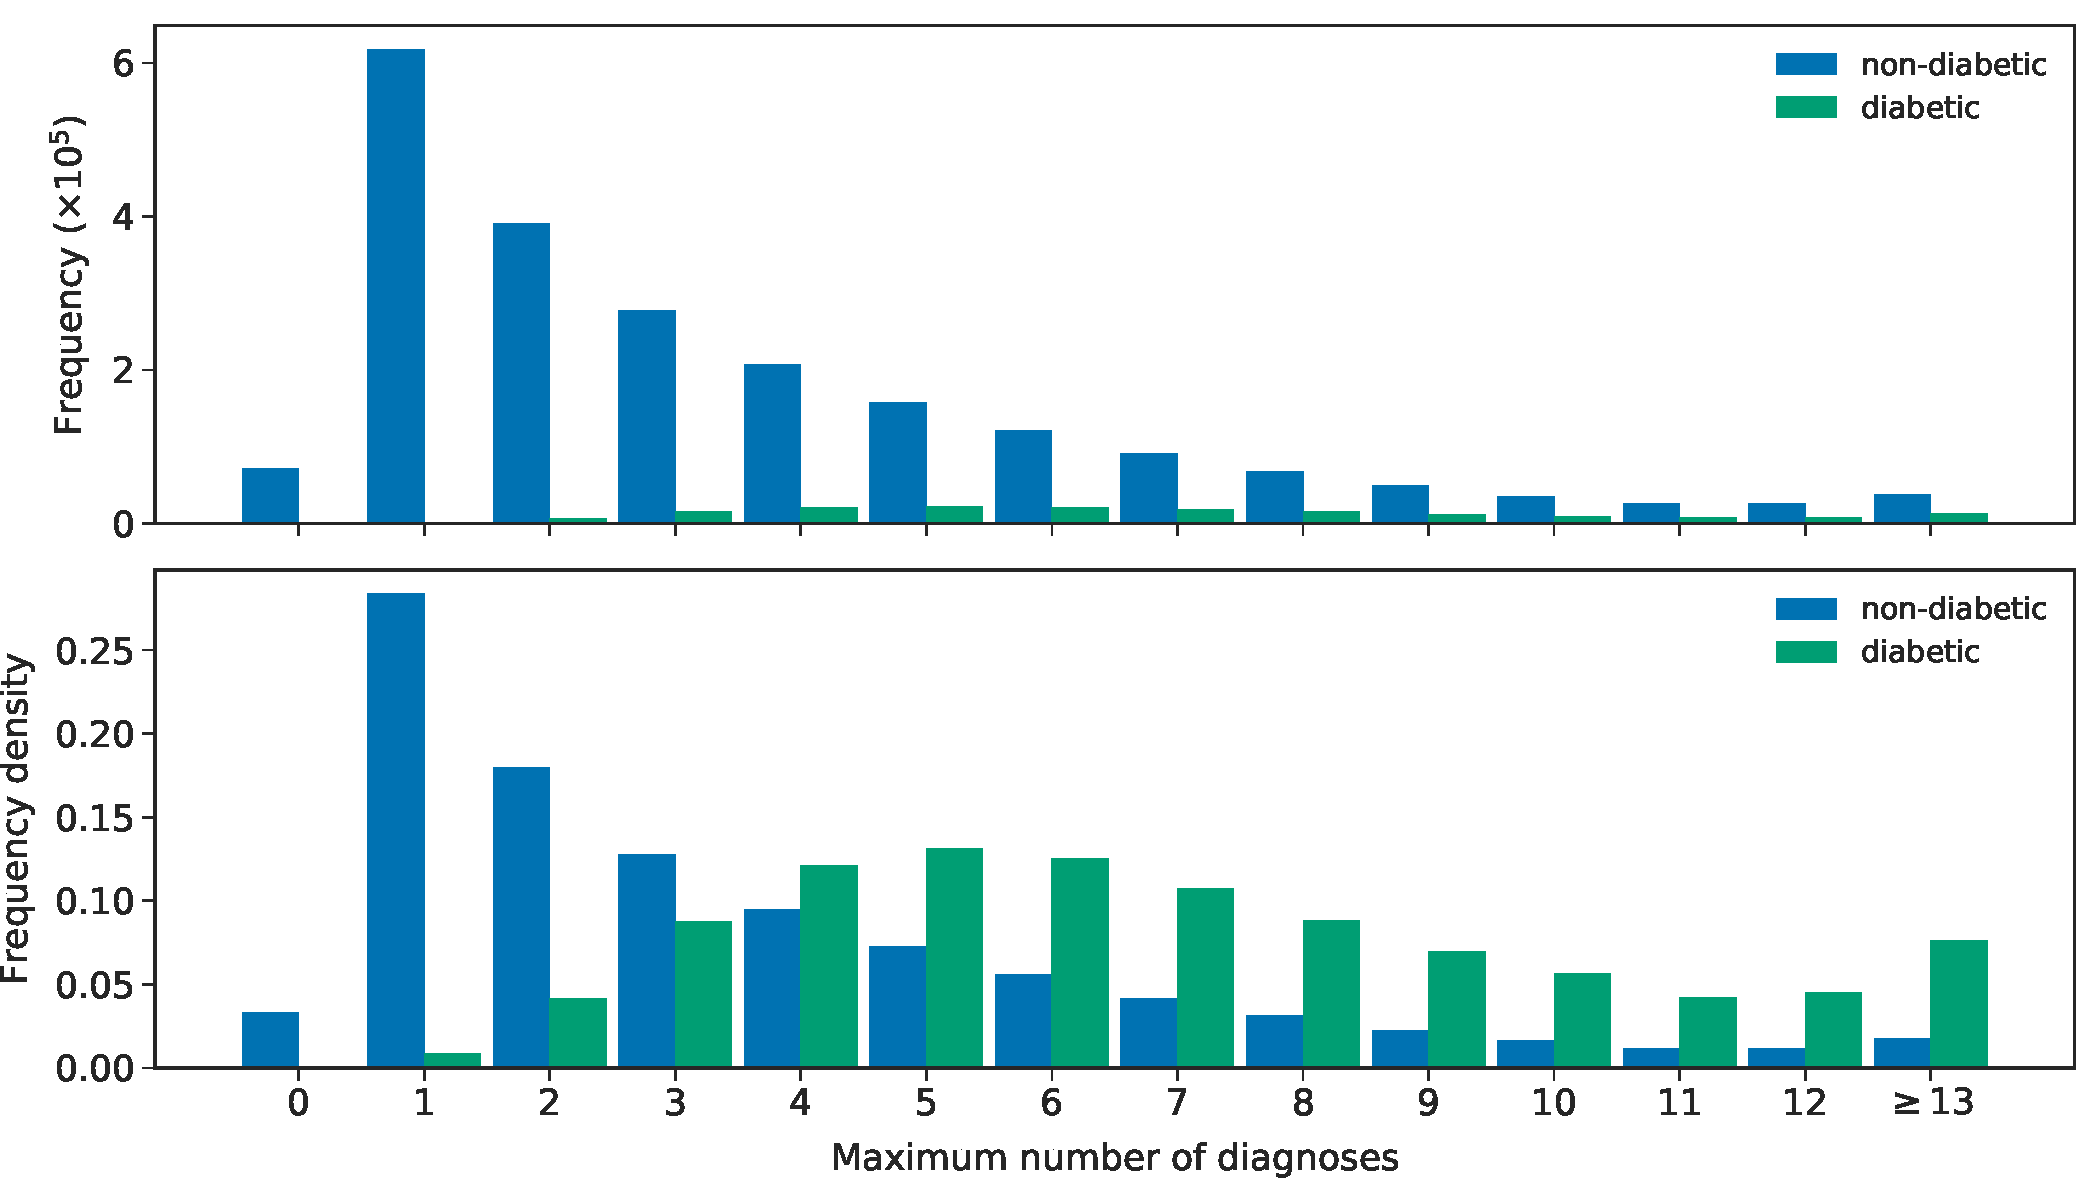
\includegraphics[width=\linewidth]{ndiag_bar.pdf}
        }
    \end{minipage}\hfill%
    \begin{minipage}{.3\linewidth}
        \centering
        \textbf{\tiny{Max.\ number of diagnoses}}
        \resizebox{\linewidth}{!}{%
            \begin{tabular}{lll}
\toprule
{} & Non-diabetic & Diabetic \\
\midrule
mean &         2.57 &     6.07 \\
std  &         8.13 &    12.55 \\
min  &         0.00 &     0.00 \\
1\%   &         0.00 &     0.00 \\
25\%  &         0.00 &     0.00 \\
50\%  &         0.00 &     1.00 \\
75\%  &         2.00 &     7.00 \\
99\%  &        35.00 &    57.00 \\
max  &       690.00 &   705.00 \\
\bottomrule
\end{tabular}

        }
    \end{minipage}\hfill%
}

\frame{\frametitle{Net costs}
    \makebox[\linewidth]{%
        \begin{minipage}{.7\linewidth}
            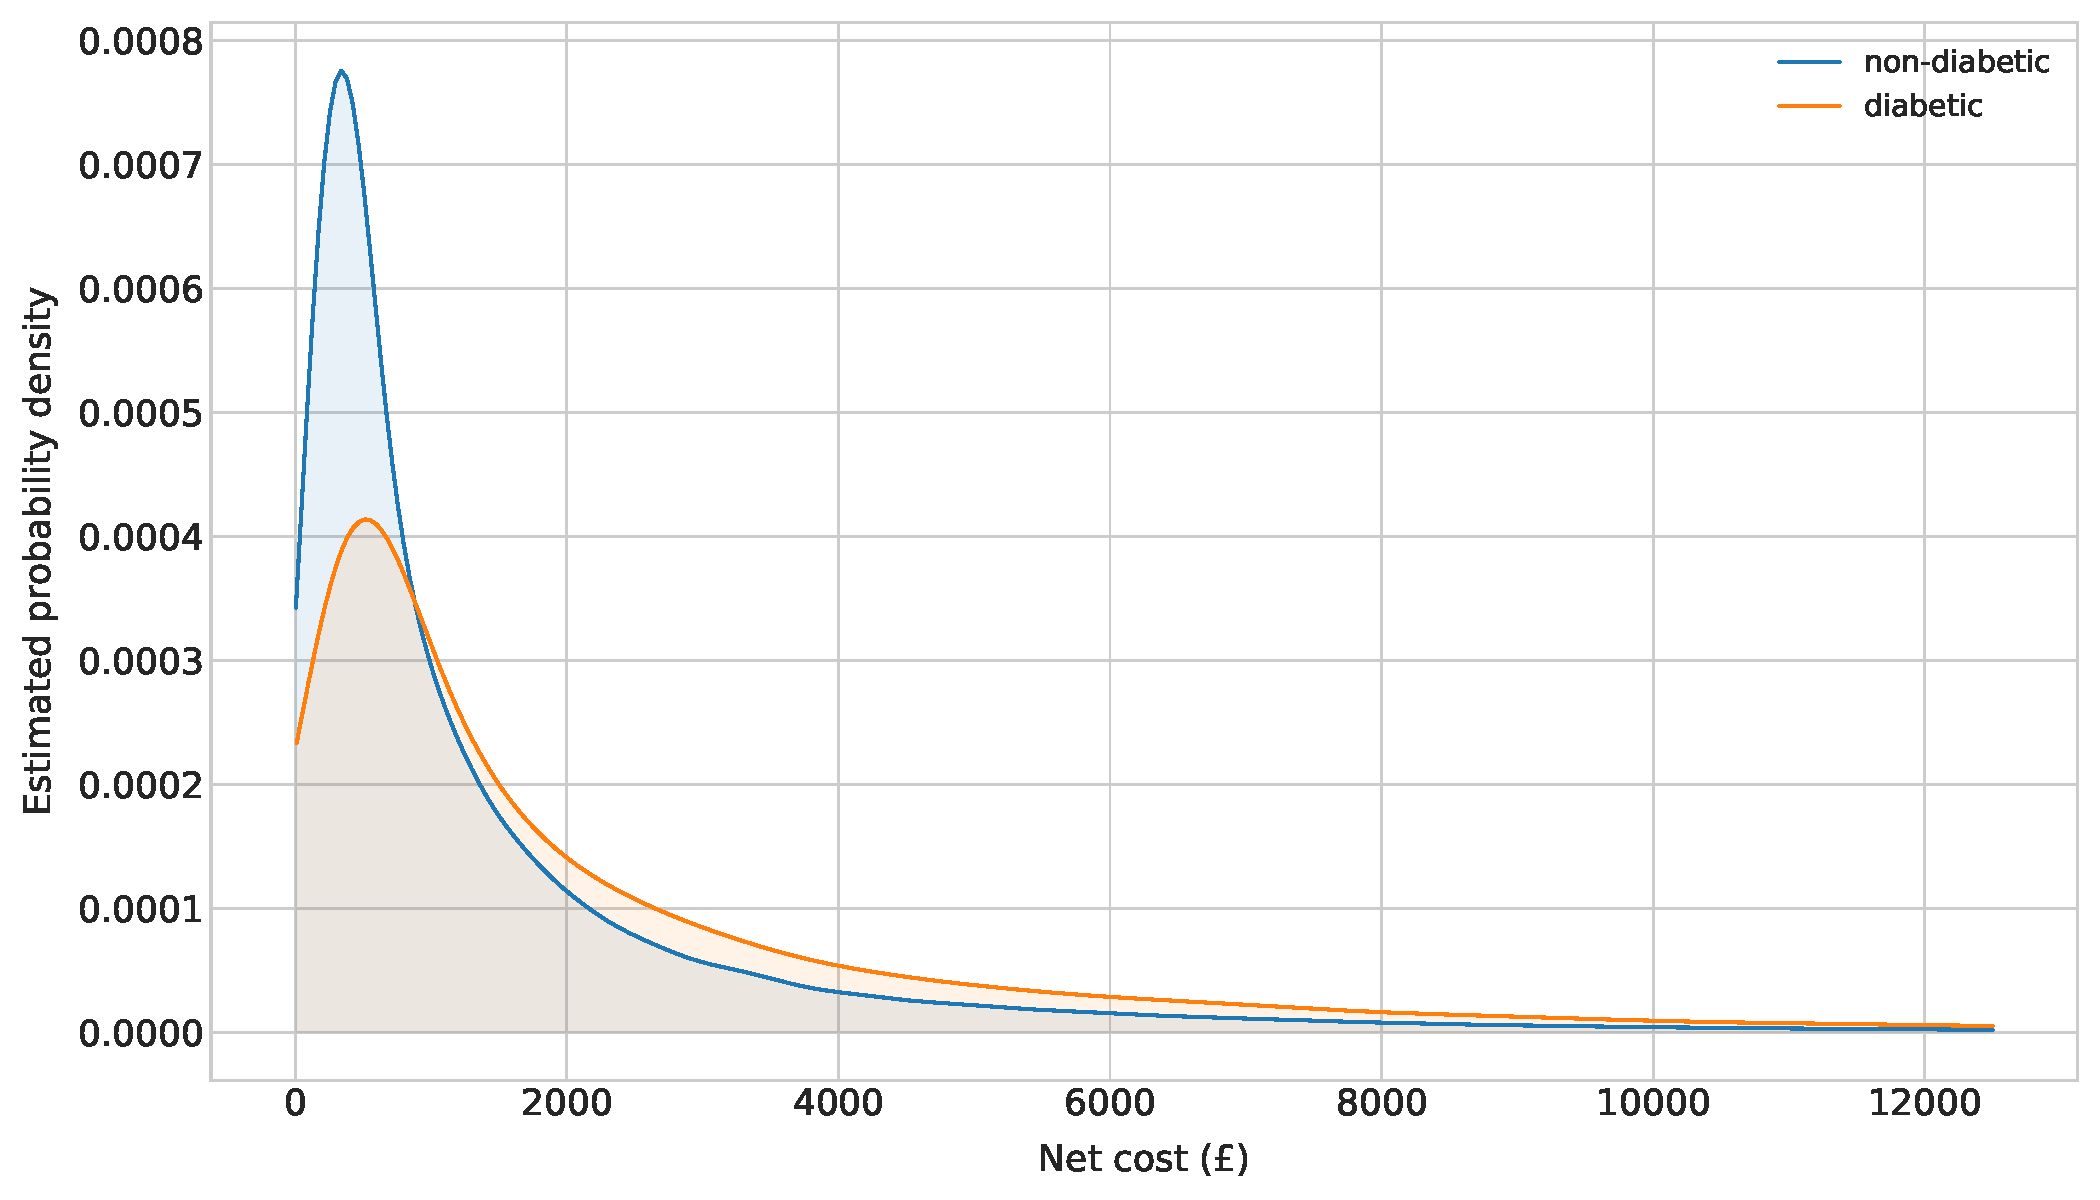
\includegraphics[width=\linewidth]{netcost_kde.pdf}
        \end{minipage}\hfill%
        \begin{minipage}{.25\linewidth}
            \centering
            \textbf{\tiny{Net cost of spell}}
            \resizebox{\linewidth}{!}{%
                \begin{tabular}{lll}
\toprule
{} & Non-diabetic &    Diabetic \\
\midrule
mean &     1,647.01 &    2,648.98 \\
std  &     3,019.54 &    4,152.20 \\
min  &         4.50 &       10.91 \\
1\%   &        62.55 &      139.65 \\
25\%  &       338.67 &      490.64 \\
50\%  &       709.33 &    1,227.95 \\
75\%  &     1,756.90 &    3,106.44 \\
95\%  &     6,179.92 &    9,591.06 \\
99\%  &    13,414.47 &   19,128.45 \\
max  &   369,168.93 &  273,450.30 \\
\bottomrule
\end{tabular}

            }
        \end{minipage}\hfill%
    }
}

\frame{\frametitle{Variation and importance}
    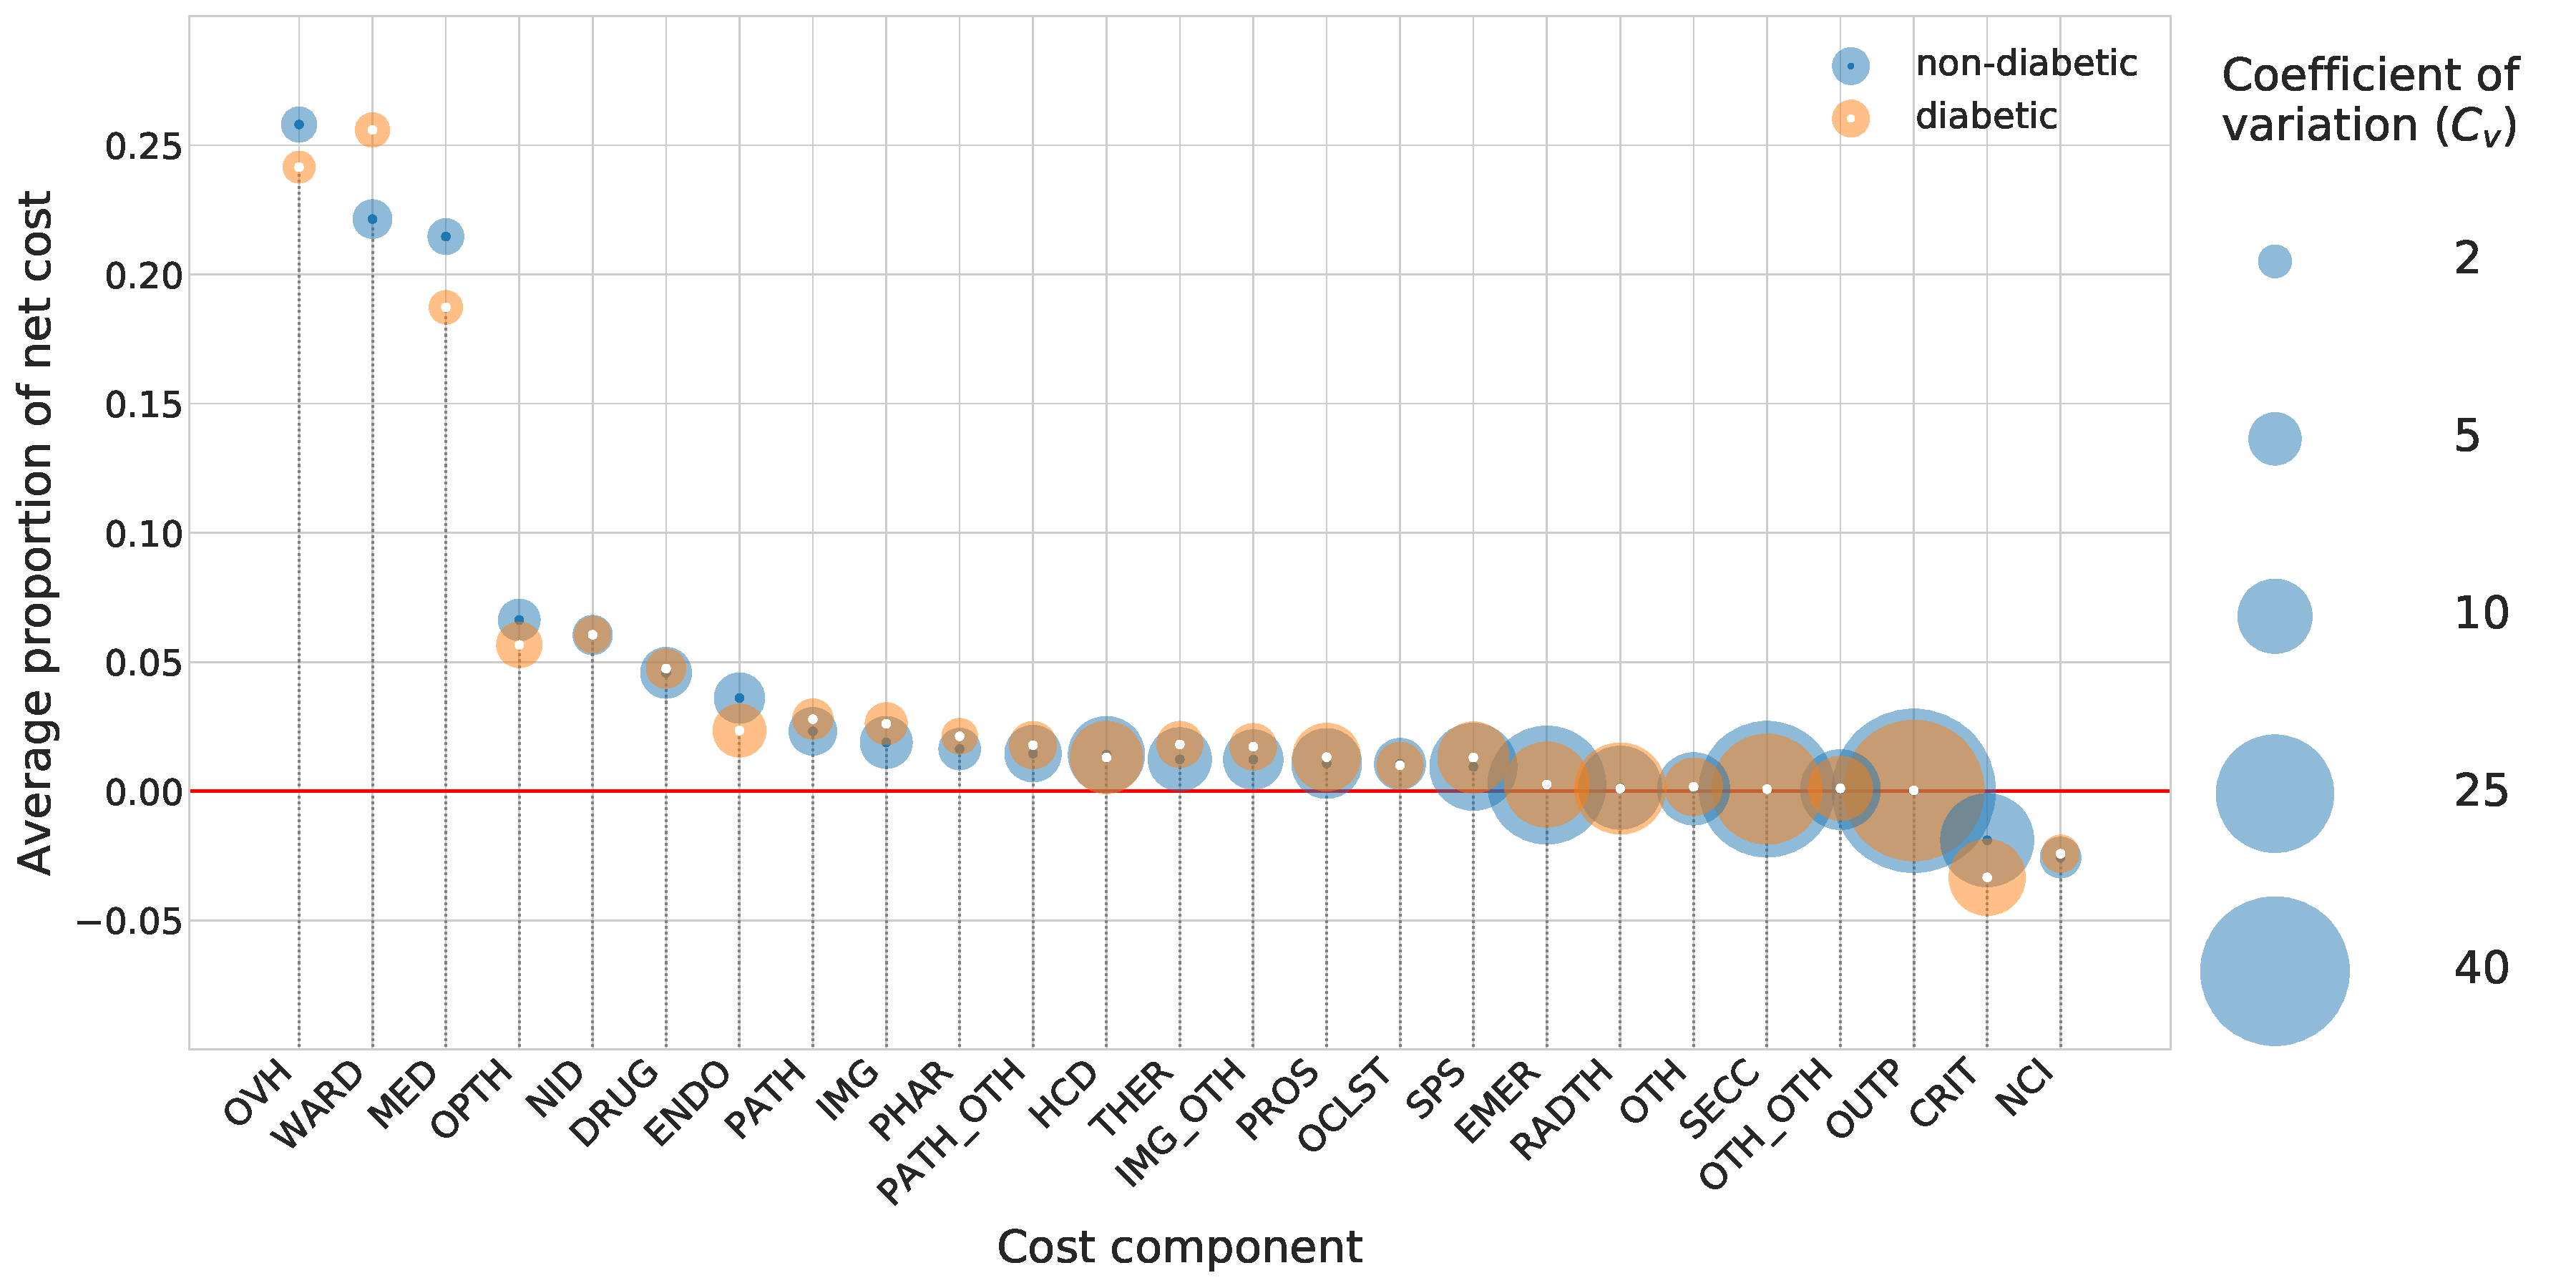
\includegraphics[width=\linewidth]{cost_bubble.pdf}
}

